\documentclass[tikz,border=10pt]{standalone}
% Pixel coordinates are used directly; y-unit is negative so the image is not flipped.
% Scale s = 0.009963 cm per pixel (STYLE METRICS), so the longest side spans 8 cm.
\usetikzlibrary{calc}
\begin{document}
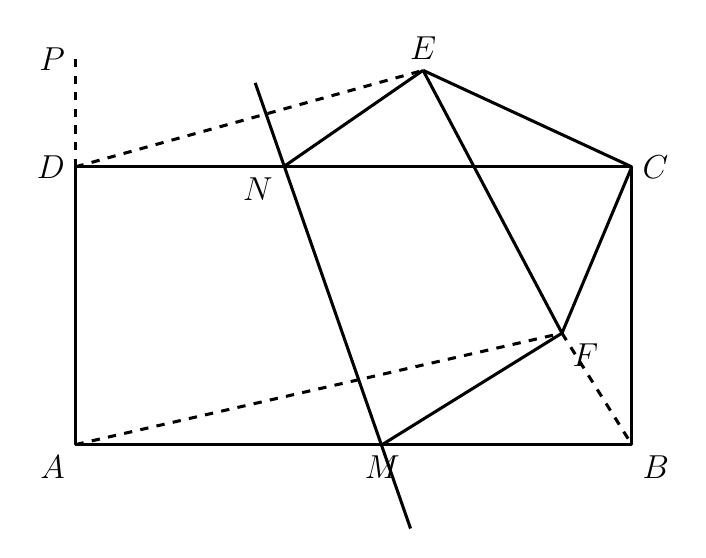
\begin{tikzpicture}[x=0.009963cm, y=-0.009963cm, line join=round, line width=1.1pt,
  every node/.style={font=\fontsize{11.5}{13.8}\selectfont}]

% Vertices (pixel coordinates)
\coordinate (A) at (105,576);
\coordinate (B) at (814,576);
\coordinate (C) at (814,222);
\coordinate (D) at (105,222);
\coordinate (P) at (105,85);
\coordinate (E) at (548,99);
\coordinate (N) at (370,222);
\coordinate (F) at (725,434);
\coordinate (M) at (496,576);

% Long solid line through N and M, extended beyond both
\draw (334,115) -- (532,683);

% Solid rectangle ABCD
\draw (A) -- (B) -- (C) -- (D) -- cycle;

% Solid edges E-N, E-C, E-F, F-C, F-M
\draw (E) -- (N);
\draw (E) -- (C);
\draw (E) -- (F);
\draw (F) -- (C);
\draw (F) -- (M);

% Dashed edges
\draw[dashed] (D) -- (P);
\draw[dashed] (D) -- (E);
\draw[dashed] (A) -- (F);
\draw[dashed] (F) -- (B);

% Labels just outside each point
\node[below left] at (A) {$A$};
\node[below right] at (B) {$B$};
\node[right] at (C) {$C$};
\node[left] at (D) {$D$};
\node[above] at (E) {$E$};
\node[below left] at (N) {$N$};
\node[below] at (M) {$M$};
\node[below right] at (F) {$F$};
\node[left] at (P) {$P$};

\end{tikzpicture}
\end{document}